\documentclass[12pt]{article}
\usepackage[a4paper, total={7in, 10in}]{geometry}
\usepackage{amsmath, amssymb}
\usepackage{graphicx, tipa}
\usepackage{wrapfig}
\usepackage[export]{adjustbox}
\usepackage{float}

\newcommand\ddfrac[2]{\frac{\displaystyle #1}{\displaystyle #2}}
\newcommand{\arc}[1]{{%
		\setbox9=\hbox{#1}%
		\ooalign{\resizebox{\wd9}{\height}{\texttoptiebar{\phantom{A}}}\cr#1}}}


\title{Circle Geometry Lesson\vspace{-3mm}}
\author{SLSS Math Club 2019\vspace{-5mm}}
\date{April 17, 2019\vspace{-5mm}}

\begin{document}
\maketitle
\section{Introduction}
The geometry of the circle represents an area of mathematics from which relatively
difficult and interesting problems for the Euclid contest are frequently taken. You are expected to know some knowledge of the elementary properties of triangles, congruence and similarity, and properties of quadrilaterals.
\section{Terminology}

\begin{itemize}
	\item \textbf{Radius(OA) - } the segment between \textbf{Center(point O)} to each point on the circle. 
	\item \textbf{Chord(AC) - } a segment whose endpoints are both on the circle. 
	\item \textbf{Diameter(AB) - } a chord which passes through the center of a circle. It is also the longest chord in a circle. 
	\item \textbf{Tangent(Line h) - } a line which touches the circle in only one place. 
	\item \textbf{Secant(Line i) - } a line which passes through the circle, intersecting it in two places.
	\item \textbf{Arc(\arc{BD}) - } the part of the curve of a circle. Since \arc{BD} can refer to two different arcs, the long and the short way around the circle, often three points are used to designate the arc, as in \arc{BAD}. 
	If only two points are used to designate an arc, it is assumed to mean the shorter one. 
\end{itemize}
\begin{figure}[h!]
\centering
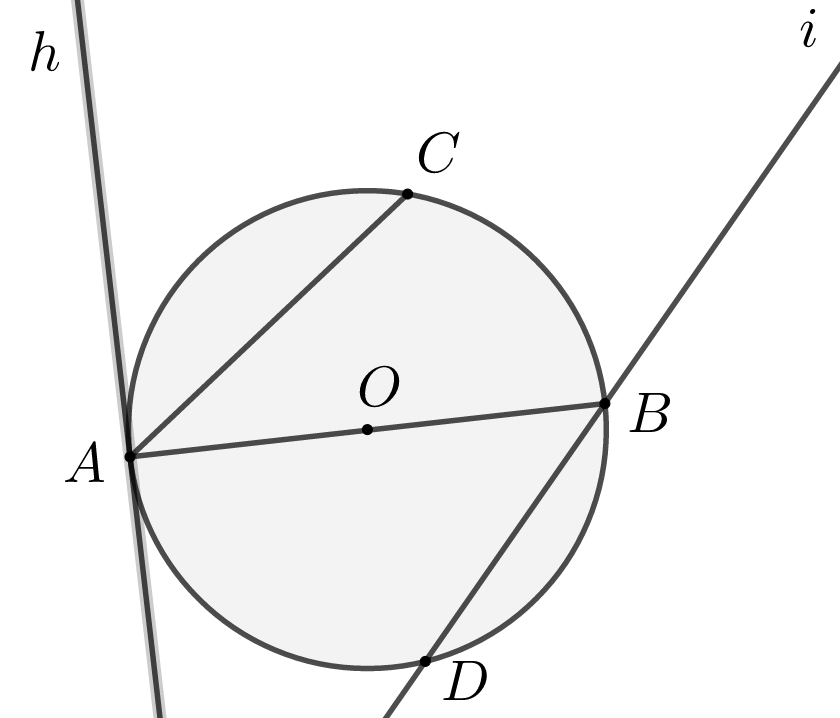
\includegraphics[width=0.3\textwidth]{Graphics/Week_13/GeometryDiagram.png}
\label{fig: 2.1}
\caption{A circle diagram}
\end{figure}

 

\pagebreak
\section{Theories}
	\subsection{Basic Formulas and Rules}
	\begin{itemize}
		\item If $d$ is the diameter of the circle, and $r$ is the radius of the circle, $d=2r$.
		\item The area of a circle, denoted by $A$, is $A=\pi r^2$.
		\item The formula for the circumference of a circle is $\pi d=2\pi r$.
		\item The formula for the arc length of a sector, denoted by "S", is calculated by $S=r\theta$, where $\theta$ is the angle between the sides of the arc, in radians. Meaning the arc length of a circle is ($\pi \cdot r$) which it is a circle's circumference.
		\item The formula to convert between degrees to radian angles is denoted by $\theta\,^{\circ}\cdot \ddfrac{\pi}{180^{\,\circ}}=\theta \, rad$.
	\end{itemize}

	\large
	\subsection{The "Star Trek" Theorem}
	The central angle subtended by any arc is twice any of the inscribed angles on that arc.
	 ($\angle AOB = 2\angle ACB$)\\
	
	\textbf{Thales' Theorem:} If a triangle is inscribed inside a circle, where one side of the triangle is the diameter of the circle, then the angle opposite to that side is a right angle.
	
	\begin{figure}[h!]
		\centering
		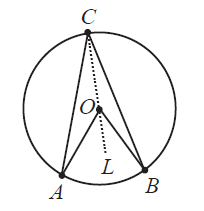
\includegraphics[height=0.15\textheight]{Graphics/Week_13/StarTreck.png}
		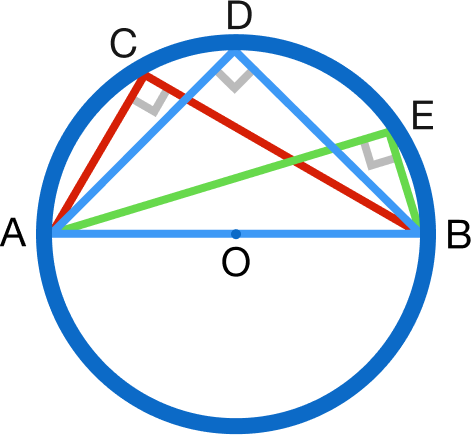
\includegraphics[height=0.15\textheight]{Graphics/Week_13/ThalesTheorem.png}
	\end{figure}
	\vspace{-5mm}
	
	\subsection{Inscribed Angles}
	The angles in the same segment from a common chord are equal.\\
	$\angle ACB = \angle ADB = \frac{1}{2}\angle AOB$
	
	\begin{figure}[h!]
		\centering
		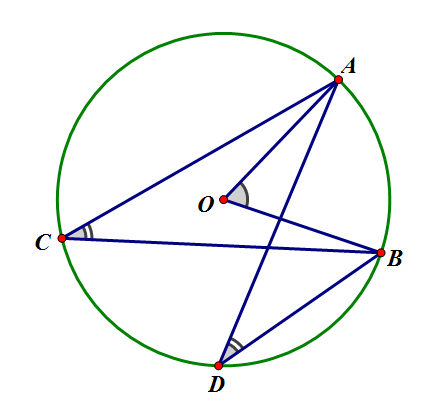
\includegraphics[height=0.2\textheight]{Graphics/Week_13/InscribedAngles.png}
	\end{figure}
	\newpage
	
	\subsection{Intersecting Chords}
	If two chords inside a circle intersect, the products of the intercepts of two intersecting chords are equal.\\ As shown in the figure below, $(PA)(PB) = (PC)(PD)$
	\begin{figure}[h!]
		\centering
		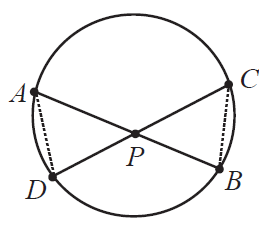
\includegraphics[height=0.2\textheight]{Graphics/Week_13/IntersectingChords.png}
	\end{figure}
	
	\subsection{Alternate Segment Theorem}
	The angle between a tangent and a chord through the point of contact is equal to the angle in the alternate segment.\\
	$\angle DCE = \angle DEB$
	\begin{figure}[h!]
		\centering
		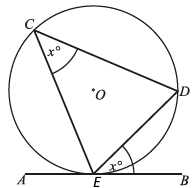
\includegraphics[height=0.2\textheight]{Graphics/Week_13/AlternateSegment.png}
	\end{figure}

	\subsection{NoName Theorem (Perpendicular, Midpoint and Bisect Chords)}
	If one of the following statements is true, the other two statements are true as well:
	\begin{enumerate}
		\item The perpendicular from the center of a circle to a chord bisects the chord.
		\item The line from the centre of a circle to the midpoint of a chord is perpendicular to the chord.
		\item The perpendicular bisector of a chord passes through the center of the circle.
	\end{enumerate}
	\begin{figure}[h!]
		\centering
		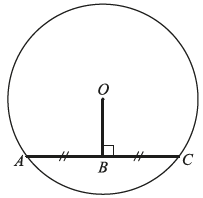
\includegraphics[height=0.2\textheight]{Graphics/Week_13/MidBisectChord.png}
	\end{figure}

	\subsection{Right Angle Tangent}
	The tangent to a circle is perpendicular to the radius drawn to the point of contact.
	$\angle OBC = 90^{\,\circ}$
	\begin{figure}[h!]
		\centering
		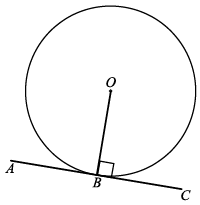
\includegraphics[height=0.2\textheight]{Graphics/Week_13/RightAngleTangent.png}
	\end{figure}

	\subsection{Equal Tangents}
	Tangents to a circle from an external point are equal.\\
	$AC=AB$
	\begin{figure}[h!]
		\centering
		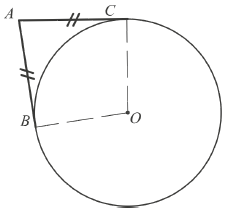
\includegraphics[height=0.2\textheight]{Graphics/Week_13/EqualTangents.png}
	\end{figure}

\newpage
\newcommand{\spacing}{\\ \\ \\ \\ \\ \\ \\ \\ \\}
\section{Practice}
	\begin{enumerate}
		\item In the diagram, the lines YZ and YX are tangents of the circle with center W. If YZ = WZ, and the the area of the quadrilaterals YZWX is 9, what is the area of the circle?  
		\begin{figure}[h!]
			\centering
			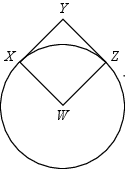
\includegraphics[height=0.2\textheight]{Graphics/Week_13/Questions/Q2.png}
		\end{figure}\\ 
	    
	    \item In a circle with centre $O$, two chords AC and BD intersect at P. Show that $\angle APB =\frac{1}{2}(\angle AOB + \angle COD)$ \spacing

	    
	    \item As shown in the diagram, a circle with centre A and radius 9 is tangent to a smaller circle with centre D and
	    radius 4. Common tangents EF and BC are drawn to the circles making points of contact at E, B and C.
	    Determine the length of EF.
	    \begin{figure}[h!]
	    	\centering
	    	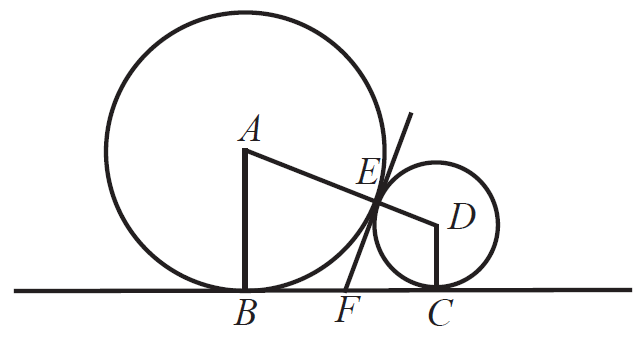
\includegraphics[height=0.2\textheight]{Graphics/Week_13/Questions/Q1.png}
	    \end{figure}
	\end{enumerate}
\end{document}